\section{Speculative Decoding for Batch Inference of LLM Agents}
\label{sec:bottleneck}
In this section, we provide a systematic efficiency analysis of large-batch speculative decoding in the LLM agent scenario. We choose the Code Generation Agent implemented by Reflexion~\citep{DBLP:conf/nips/ShinnCGNY23} and tested on USACO dataset~\citep{DBLP:journals/corr/abs-2404-10952} as the agent workload for analysis. To ensure a fair and realistic analysis, we deploy the LLM of the agent application in vLLM~\citep{DBLP:conf/sosp/KwonLZ0ZY0ZS23}, one of the production-ready LLM serving engines and select two representative speculative decoding algorithms that cover two main types as mentioned in~\cref{subsec:specualtive_decoding}, including the draft-model-based method EAGLE-3~\citep{DBLP:journals/corr/abs-2503-01840} and the draft-model-free method NGram~\citep{saxena2023prompt}. Following the standard of previous work~\citep{DBLP:conf/sosp/KwonLZ0ZY0ZS23}, we choose the total token number generated divided by the total execution time of the workload as the throughput metric for efficiency evaluation.

% 我第一个说Bottleneck of High Rejection Rate，然后先建模enhancement of accept number / cost of reject number with bz，然后记录inference时候plot rejection number vs. accept number per instance和avearge rejection cost vs avearge accept saving with bz 可以么, 然后第二个说Bottleneck of Token Budget Under-Utilization，然后define max budget under various bz, 然后记录并plot max budget vs actual average draft token number可以么？有什么建议或者问题
\subsection{Overall Efficiency Analysis} We first compare the throughput speedup of two representative speculative decoding methods for code generation agents under varying maximum batch sizes in the vLLM engine. The results are shown in~\cref{fig:moti_bz}. When the maximum batch size is 1, EAGLE-3 achieves over $2.5\times$ speedup and SuffixDecoding achieves over $1.9\times$ speedup, consistent with consensus that speculative decoding is effective under small batch sizes. However, as the batch size increases, the speedup rapidly diminishes. When the maximum batch size exceeds 32, speculative decoding even becomes slower than standard autoregressive decoding, indicating that existing speculative decoding methods scale poorly to large-batch agent serving scenarios.

\begin{figure}[t]
\centering
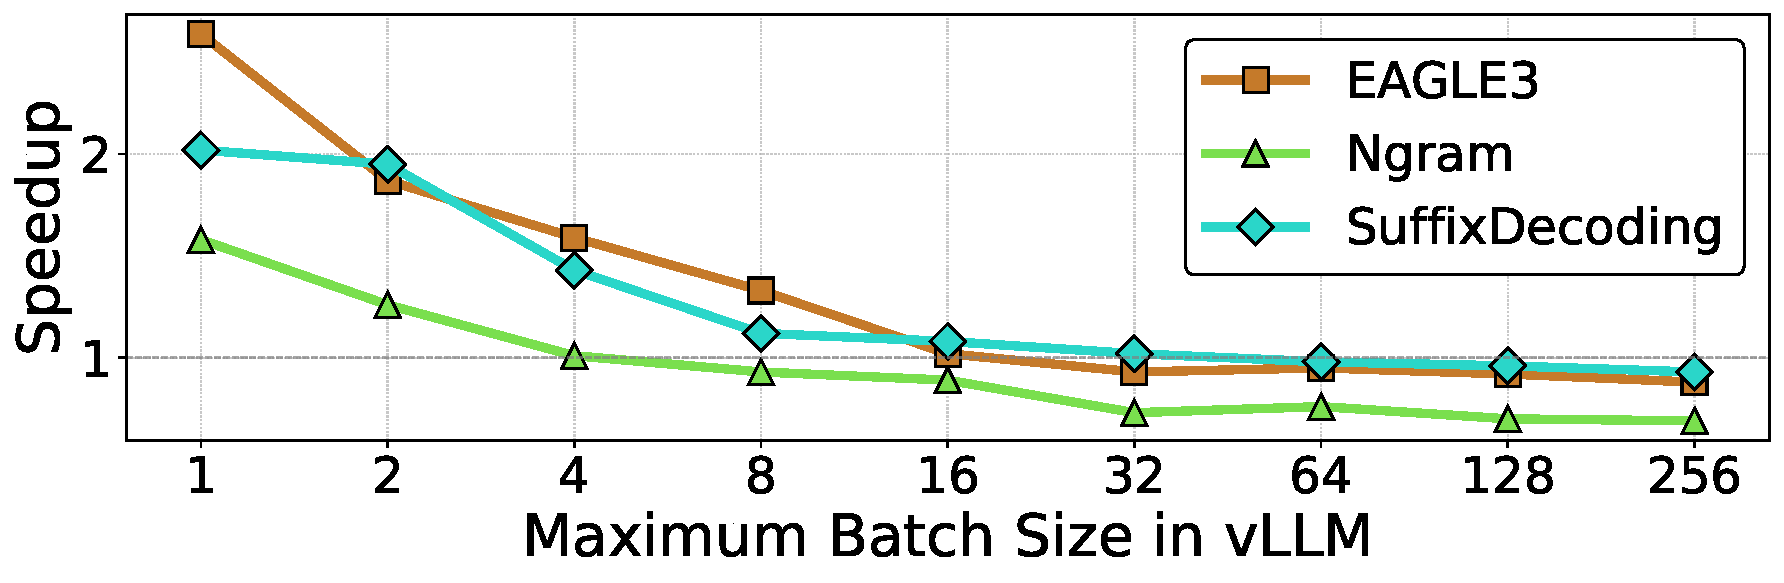
\includegraphics[width=0.48\textwidth]{Figures/moti_bz.pdf}
\caption{Speedup in terms of Goodput (number of generated tokens divided by the execution time)~\citep{liu2024optimizing} under various maximum batch size in vLLM for different speculative decoding algorithms on USACO dataset with Code Generation Agent implemented by Reflexion agentic workflow on Qwen-3-8B. }
\label{fig:moti_bz}
\end{figure}

To understand the cause of this degradation, we model the per-step execution time saving $\Delta T(b)$ of speculative decoding with batch size $b$ as:
\begin{align*}
\Delta T(b) &= T_{\text{base}}(b) - T_{\text{spec}}(b) \\
&\approx D(b)(1-\rho(b))t_A - D(b)\big(t_D(b) + t_V(b)\big) \\
&= D(b)\left[(1-\rho(b))t_A - t_D(b) - t_V(b)\right] \\
&\approx D(b)\left[(1-\rho(b))t_A - t_V(b)\right]
\end{align*}
where $D(b)$ denotes the number of drafted tokens in the current step, $\rho(b)$ is the rejection rate that is defined as the ratio of rejected tokens to proposed tokens for each request in the batch, $t_A$ is the per-token time saved by accepting a draft token, and $t_D(b)$ and $t_V(b)$ are the per-token draft and verification costs.

Since $t_D(b)$ is small and can be ignored, this formulation highlights two key factors that impact the efficiency: the rejection rate $\rho(b)$ and $D(b)\big(t_A - t_V(b)\big)$, which we call the utilization of the draft token budget. In general lower rejection rates and higher budget utilization bring in an ideal speculative decoding with larger speedups.


\subsection{Bottleneck Analysis} Motivated by the analysis above, we next examine how existing methods behave with respect to the rejection rate and the token budget utilization.

\noindent\textbf{Bottleneck of High Rejection Rate.} We record the rejection rate, defined as the ratio of rejected tokens to proposed tokens for each request in the batch from vLLM logs during Code Generation Agent inference. ~\cref{tab:rejection_rate} records the average rejection rate for different speculative decoding algorithms. As shown, existing speculative decoding methods suffer from extremely high rejection rates: EAGLE-3 exceeds 50\%, while NGram exceeds 85\% across most batch sizes. Such high rejection rates substantially limit the effective utilization of the draft token budget, directly contributing to the observed degradation in throughput speedup under large-batch settings for LLM agent inference.

\rejTable

\noindent\textbf{Bottleneck of Token Budget Under-Utilization.} We define the available token budget under batch size $b$ as $M(b) = AI - b$, where $AI$ denotes the arithmetic intensity of the deployed hardware for the LLM agent. This definition reflects the fact that, as the batch size increases, LLM inference—particularly the FFN layers—quickly becomes compute-bound and dominates end-to-end latency. As a result, the verification cost $t_V(b)$ increases and eventually approaches the per-token acceptance saving $t_A$, making the total execution time saving $\Delta T(b)$ become:
\begin{align*}
\Delta T(b)
&\approx D(b)\left[(1-\rho(b)) t_A - t_V(b)\right] \\
&= D(b)\left[(1-\rho(b)) t_A - t_A\right] = -D(b)\rho(b) t_A < 0
\end{align*}


\begin{figure}[t]
\centering
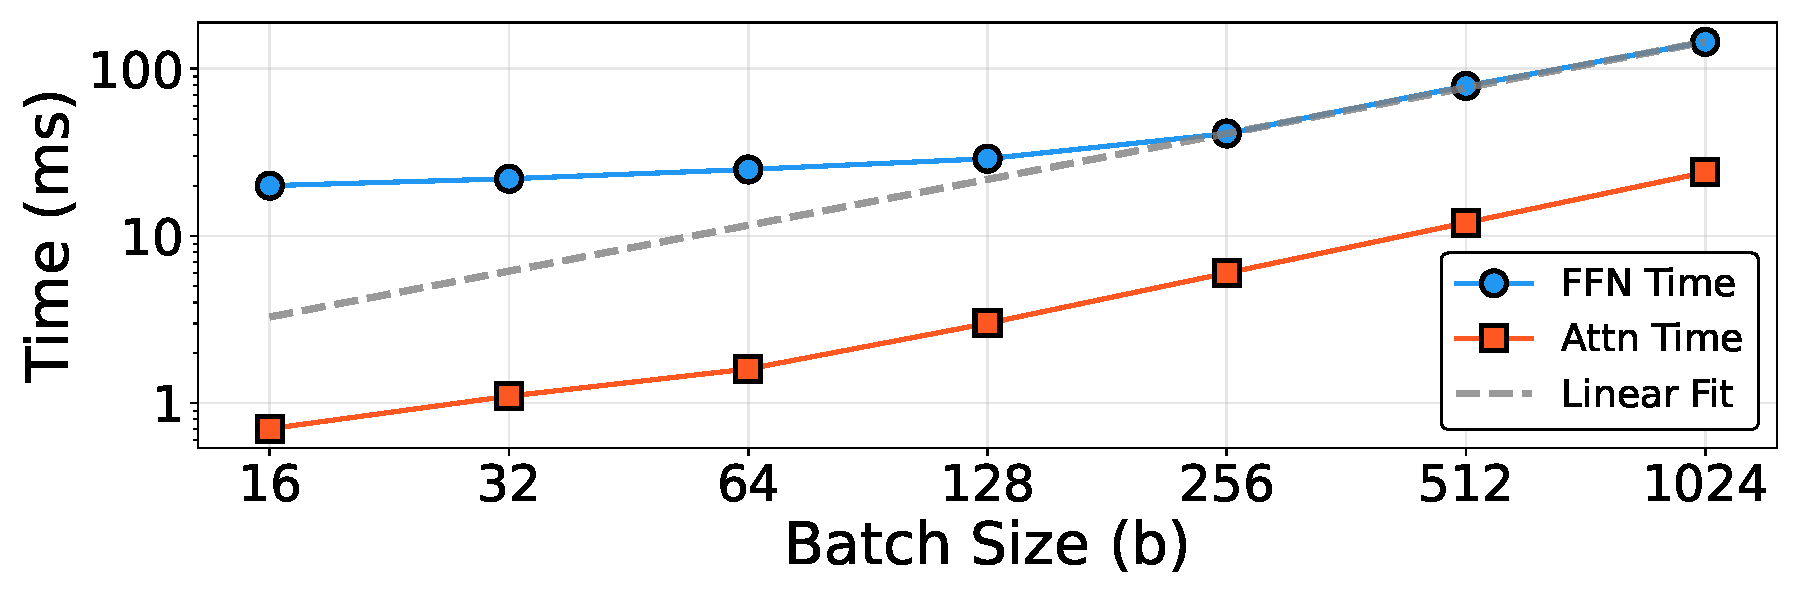
\includegraphics[width=0.48\textwidth]{Figures/moti_ffn_attn.pdf}
\caption{Execution time comparison for FFN and Attention modules of Qwen-3-8B under various batch size. }
\label{fig:moti_ffn_attn}
\end{figure}
To further illustrate this effect, we measure the per-layer decoding time of the FFN and attention modules of Qwen-3-8B using vLLM with FlashAttention-2 on an A100 GPU. The results are shown in~\cref{fig:moti_ffn_attn}. When the batch size exceeds 256, which matches the arithmetic intensity of the A100, the FFN latency grows linearly with batch size and quickly dominates the total decoding time. In this regime, decoding becomes compute-bound by the FFN, and the per-token verification cost $t_V(b)$ approaches the per-token autoregressive decoding cost $t_A$. As a result, the time saved by accepting one draft token is almost entirely offset by the cost of verifying it, leaving speculative decoding with little or no performance gain. This observation justifies our definition of the available token budget $M(b)$, which captures the diminishing headroom for speculative tokens as batch size increases.

\begin{figure}[t]
\centering
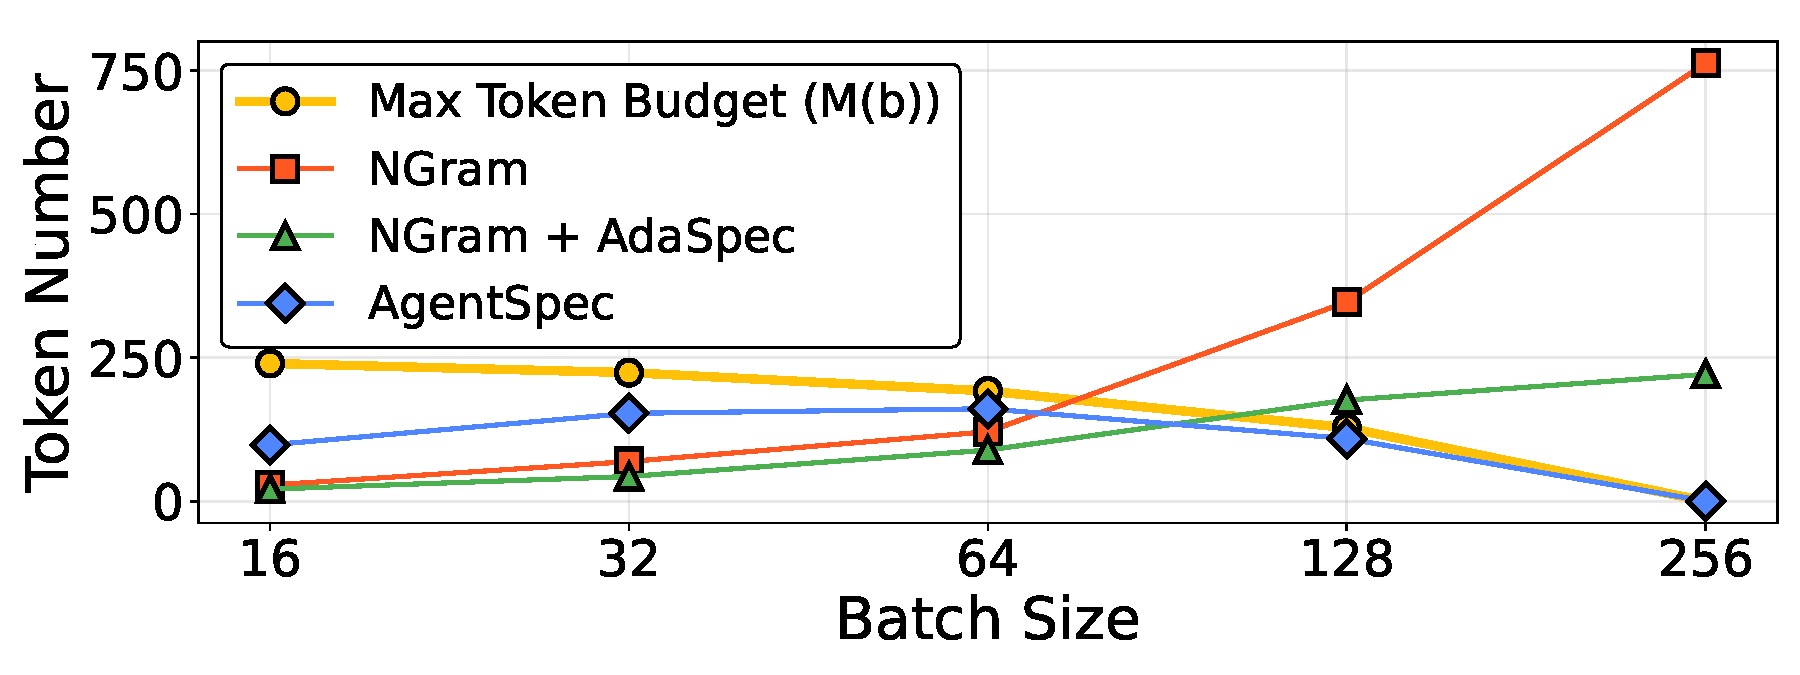
\includegraphics[width=0.48\textwidth]{Figures/moti_token_number.pdf}
\caption{Comparison between maximum token budget $M(b)$ and average proposed token number for batch inference of speculative decoding on Reflexion workflow.}
\label{fig:moti_token_number}
\end{figure}
We next record the total number of draft tokens generated per decoding step under different batch sizes and compare it with the available token budget $M(b)$. For a fair comparison, we also implement the budget allocation strategy from AdaSpec~\citep{10.1145/3772052.3772239}, which assigns draft tokens based on per-request acceptance rates. As shown in~\cref{fig:moti_token_number}, we have two key findings. (1) Existing speculative decoding methods severely under-utilize the available token budget, with the actual draft token count remaining far below or over $M(b)$ across all batch sizes.
(2) Existing allocation strategy fails to improve budget utilization, indicating that acceptance-rate–based budgeting is ineffective to improve the batch inference of speculative decoding for LLM agent.
% define max budget under various bz, budget vs draft tk ct
% solution: accept rate: 
